\section{Methods}
\pgfdeclareimage[width=1.0\paperwidth]{header-image}{header_images/Sierra_Calderona}

\def \inputMap#1#2#3#4 {
    \begin{backgroundblock}{#1}{#2}
        \begin{tikzpicture}
            \node[anchor=south west,inner sep=0] (image) at (0,0) {
                \includegraphics[width=4.0cm]{images/inputs/#3}
            };
            \node[align=center, font = {\tiny}] at (2.15cm, 2.33cm) {#4};
        \end{tikzpicture}
    \end{backgroundblock}
}

\def \inputMapA#1#2 {
    \inputMap{5cm}{1.33cm}{#1}{#2}
}
\def \inputMapB#1#2 {
    \inputMap{6.67cm}{3.67cm}{#1}{#2}
}
\def \inputMapC#1#2 {
    \inputMap{8.33cm}{6cm}{#1}{#2}
}

\begin{frame}<2-5, 7-8>[label=framework]
    \frametitle{Fire limitation framework}
    \framesubtitle{Spatial and Temporal controls on burnt area}

    \begin{tikzpicture}
        \visible<2->{\fill[blue , opacity = 0.7] (90:4) -- (210:4) -- (-30:4) -- cycle;}
        \visible<3->{\fill[green,path fading=south, opacity = 0.85] (90:4) -- (210:4) -- (-30:4) -- cycle;}
        \visible<4->{\fill[red  ,path fading=west, opacity = 0.7] (90:4) -- (210:4) -- (-30:4) -- cycle;}

       
        \visible<2>{
            \node (note) at (0, 1.5em) {\Huge Moisture Content};
            \node (note) at (0, 0.0em) {\large Canopy cover};
            \node (note) at (0,-1.5em) {\large Live Fuel};
            \node (note) at (0,-3.0em) {\large Atmosphere};
        }

        \visible<3->{
            \node[rotate = 30] at (-2.5, -1.3) {\large Moisture};
        }
    
	     \visible<3>{
	    	\node (note) at (0,1.5em) {\Huge Fuel Continuity};
	    	\node (note) at (0,0) {\large Vegetative Cover};
	    }
	    
	   % \visible<4->{
	   % 	\node[rotate = -30] at (2.6,-1.3) {\large Fuel};
	    %	\node[rotate = -30] at (2.4,-1.6) {NPP};
	   % }	
    
	    \visible<4->{
	    	\node[anchor = east, rotate = 90] at (0, 3.3) {\large Fuel};
	    }
    
        \visible<4>{
            \node (note) at (0,1.5em) {\Huge Ignitions};
            \node (note) at (0,0) { \large Lightning};
            \node (note) at (0,-1.25em) { \large Population Density};
            \node (note) at (0,-2.5em) { \large Pasture};
        }

        \visible<5->{
           \node[rotate = -30] at (2.5, -1.3) {\large Ignitions};
        }

        \visible<5>{
            \node (note) at (0,0) {\Huge Burnt Area};
        }

    \end{tikzpicture}

    \begin{textblock*}{5cm}(6.67cm,2cm)
        \visible<7->{
            \begin{tikzpicture}[scale=0.67]
                \fill[green] (90:4) -- (210:4) -- (-30:4) -- cycle;
                \fill[blue,path fading=west] (90:4) -- (210:4) -- (-30:4) -- cycle;
                \fill[red,path fading=south] (90:4) -- (210:4) -- (-30:4) -- cycle;
                \fill[black, opacity = 0.3] (90:4) -- (210:4) -- (-30:4) -- cycle;
            \end{tikzpicture}
        }
    \end{textblock*}

    \begin{textblock*}{5cm}(10.1cm,2cm)
        \visible<7->{
            \begin{tikzpicture}[scale=0.33]
                \fill[green] (90:4) -- (210:4) -- (-30:4) -- cycle;
                \fill[blue,path fading=west] (90:4) -- (210:4) -- (-30:4) -- cycle;
                \fill[red,path fading=south] (90:4) -- (210:4) -- (-30:4) -- cycle;
                \fill[black, opacity = 0.5] (90:4) -- (210:4) -- (-30:4) -- cycle;
            \end{tikzpicture}
        }
    \end{textblock*}

    \begin{textblock*}{4.5cm}(4.6cm,2.6cm)
        \visible<7->{
            
\begin{tikzpicture}
                \node[rotate = 25 ] (note) at (3.335, 2.165) {\Huge Human Suppression};
                    \node[rotate = 25 ] (note) at (3.335, 1.165) {\Large Crop land, Population Density};
                \draw[ultra thick, ->] (0, 0) -- (6.67, 3.33);
            \end{tikzpicture}
        }
    \end{textblock*}

	\only<2> {
        \inputMapA{inputs_mean-npp}{Tree cover (VCF)}
		\inputMapB{inputs_mean-emc}{Equilibrium Fuel Moisture Content (Kelley et al. 2014)}
		\inputMapC{inputs_mean-alpha}{$\alpha$ (STASH: Whitley et al 2014; Davis et al 2016)}
	}%{5cm}{1.18cm}


    \only<3> {
        \inputMapA{inputs_mean-npp}{Veg cover (VCF)}
		\inputMapB{inputs_mean-alpha}{$\alpha$ (STASH: Whitley et al 2014; Davis et al 2016)}
    }

    \only<4> {        
        \inputMapA{inputs_mean-Lightn}{LIS/OTD (Christian 1999)}
        \inputMapB{inputs_mean-popdens}{HYDE Popdens (Goldewijk  et al 2011)}
        \inputMapC{inputs_mean-pas}{HYDE Pasture (Goldewijk et al 2011)}
    }

	\only<7> {
		\inputMap{4.7cm}{1.33cm}{inputs_mean-popdens}{HYDE Popdens (Goldewijk et al 2011)}
		\inputMap{8.33cm}{6cm}{inputs_mean-crop}{HYDE crop (Goldewijk et al 2011)}
	}

    \only<5> {
    	\begin{backgroundblock}{4.2cm}{1.33cm}
    		\begin{tikzpicture}
		         \node[anchor=south west,inner sep=0] (image) at (0,0) {
		        	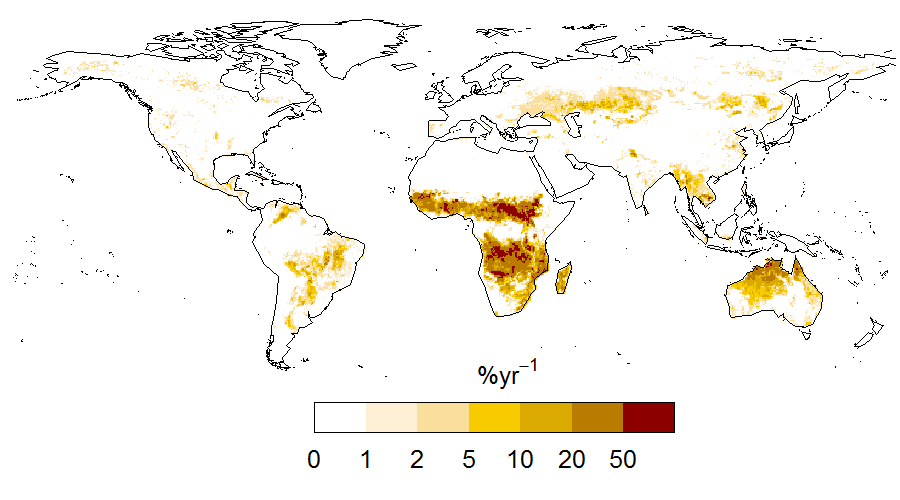
\includegraphics[width=7.0cm]{images/inputs/inputs_mean-fire}
		        };
		        \node[align=center, font = {\small}] at (2.95cm, 4.2cm) {Global Fire Emission Database 4s \\ (Giglio et al 2013; Randerson et al 2012)};
	        \end{tikzpicture}
	    \end{backgroundblock}
        %?% Make bigger
    }
    %?% Stuff to include:
    %?%   Monthly -> Inter annual and seasonal controls
\end{frame}

\def \controlsSide#1 {
    \begin{textblock*}{11cm}(0cm,1.5cm)
        \begin{tikzpicture}
            \node[anchor=south west,inner sep=0] (image) at (0,0) {
                \includegraphics[width=13.0cm]{images/#1}
            };
            \visible<-4> {\draw[white, fill = white] (6.5,3.0) -- (13.0,3.0) -- (13.0,7) -- (6.5,7) -- (6.5,3.0);}
            \visible<-1> {\draw[white, fill = white] (0.0,0.0) -- ( 6.5,0.0) -- ( 6.5,3.5) -- (0.0,3.5) -- (0.0,0.0);}
           \visible<-4>  {\draw[white, fill = white] (6.5,3.0) -- (13.0,3.0) -- (13.0,0.0) -- (6.5,0.0) -- (6.5,3.0);}
            %\visible<-4> {\draw[white, fill = white] (0.0,0) -- (12.0,0) -- (12.0,1.0) -- (0.0,1.0) -- (0.0,0);}
        \end{tikzpicture}
    \end{textblock*}
    \begin{textblock*}{11cm}(2.0cm, 7.5cm)
        \includegraphics[width=5.0cm]{images/#1_legend}
    \end{textblock*}
}

\pgfdeclareimage[width=1.0\paperwidth]{header-image}{header_images/kata_tjuta}

\def \controlsLines[#1]#2 {
\begin{frame}
	\frametitle{Controls on fire}
	\framesubtitle{Which is more important}
	\begin{textblock*}{12cm}(0.1cm,1.4cm)
        \includegraphics[width=8cm, height=7.0cm,trim={0 1.9cm 0 0}, clip]{images/limitCurves/#1}
    \end{textblock*}
    \begin{textblock*}{14cm}(7.6cm,1.2cm)
		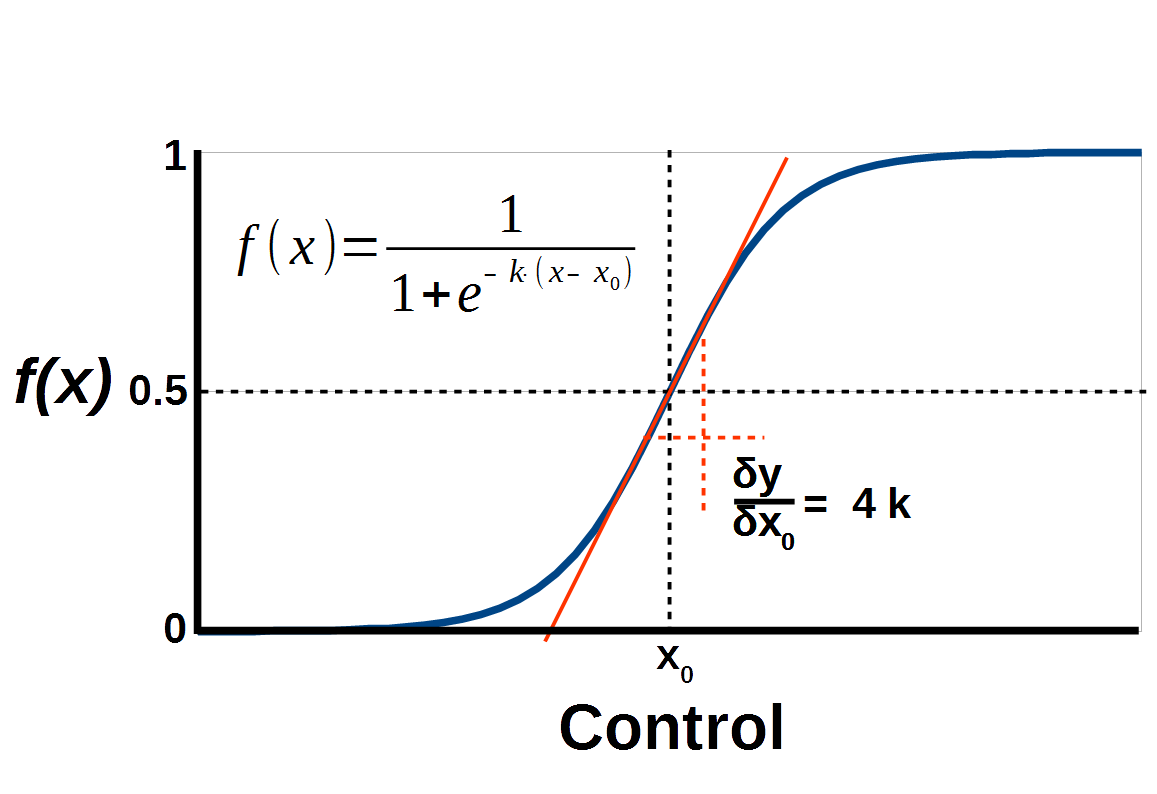
\includegraphics[width=5cm, height=4cm]{../diagrams/Logistic_fun.png}		
	\end{textblock*}
    \begin{textblock*}{14cm}(7.5cm,5.3cm)
		\includegraphics[width=5.3cm]{images/limitCurves/#2}		
	\end{textblock*}
\end{frame}
}

\controlsLines[limLines--empty]{fireMap}
\controlsLines[limLines-Desert-]{Desert/fireMap}

\controlsLines[limLines]{fireMap}
\begin{frame}
	\frametitle{Controls on fire}
	\framesubtitle{Which is more important}
	\begin{textblock*}{12cm}(0.1cm,1.4cm)
        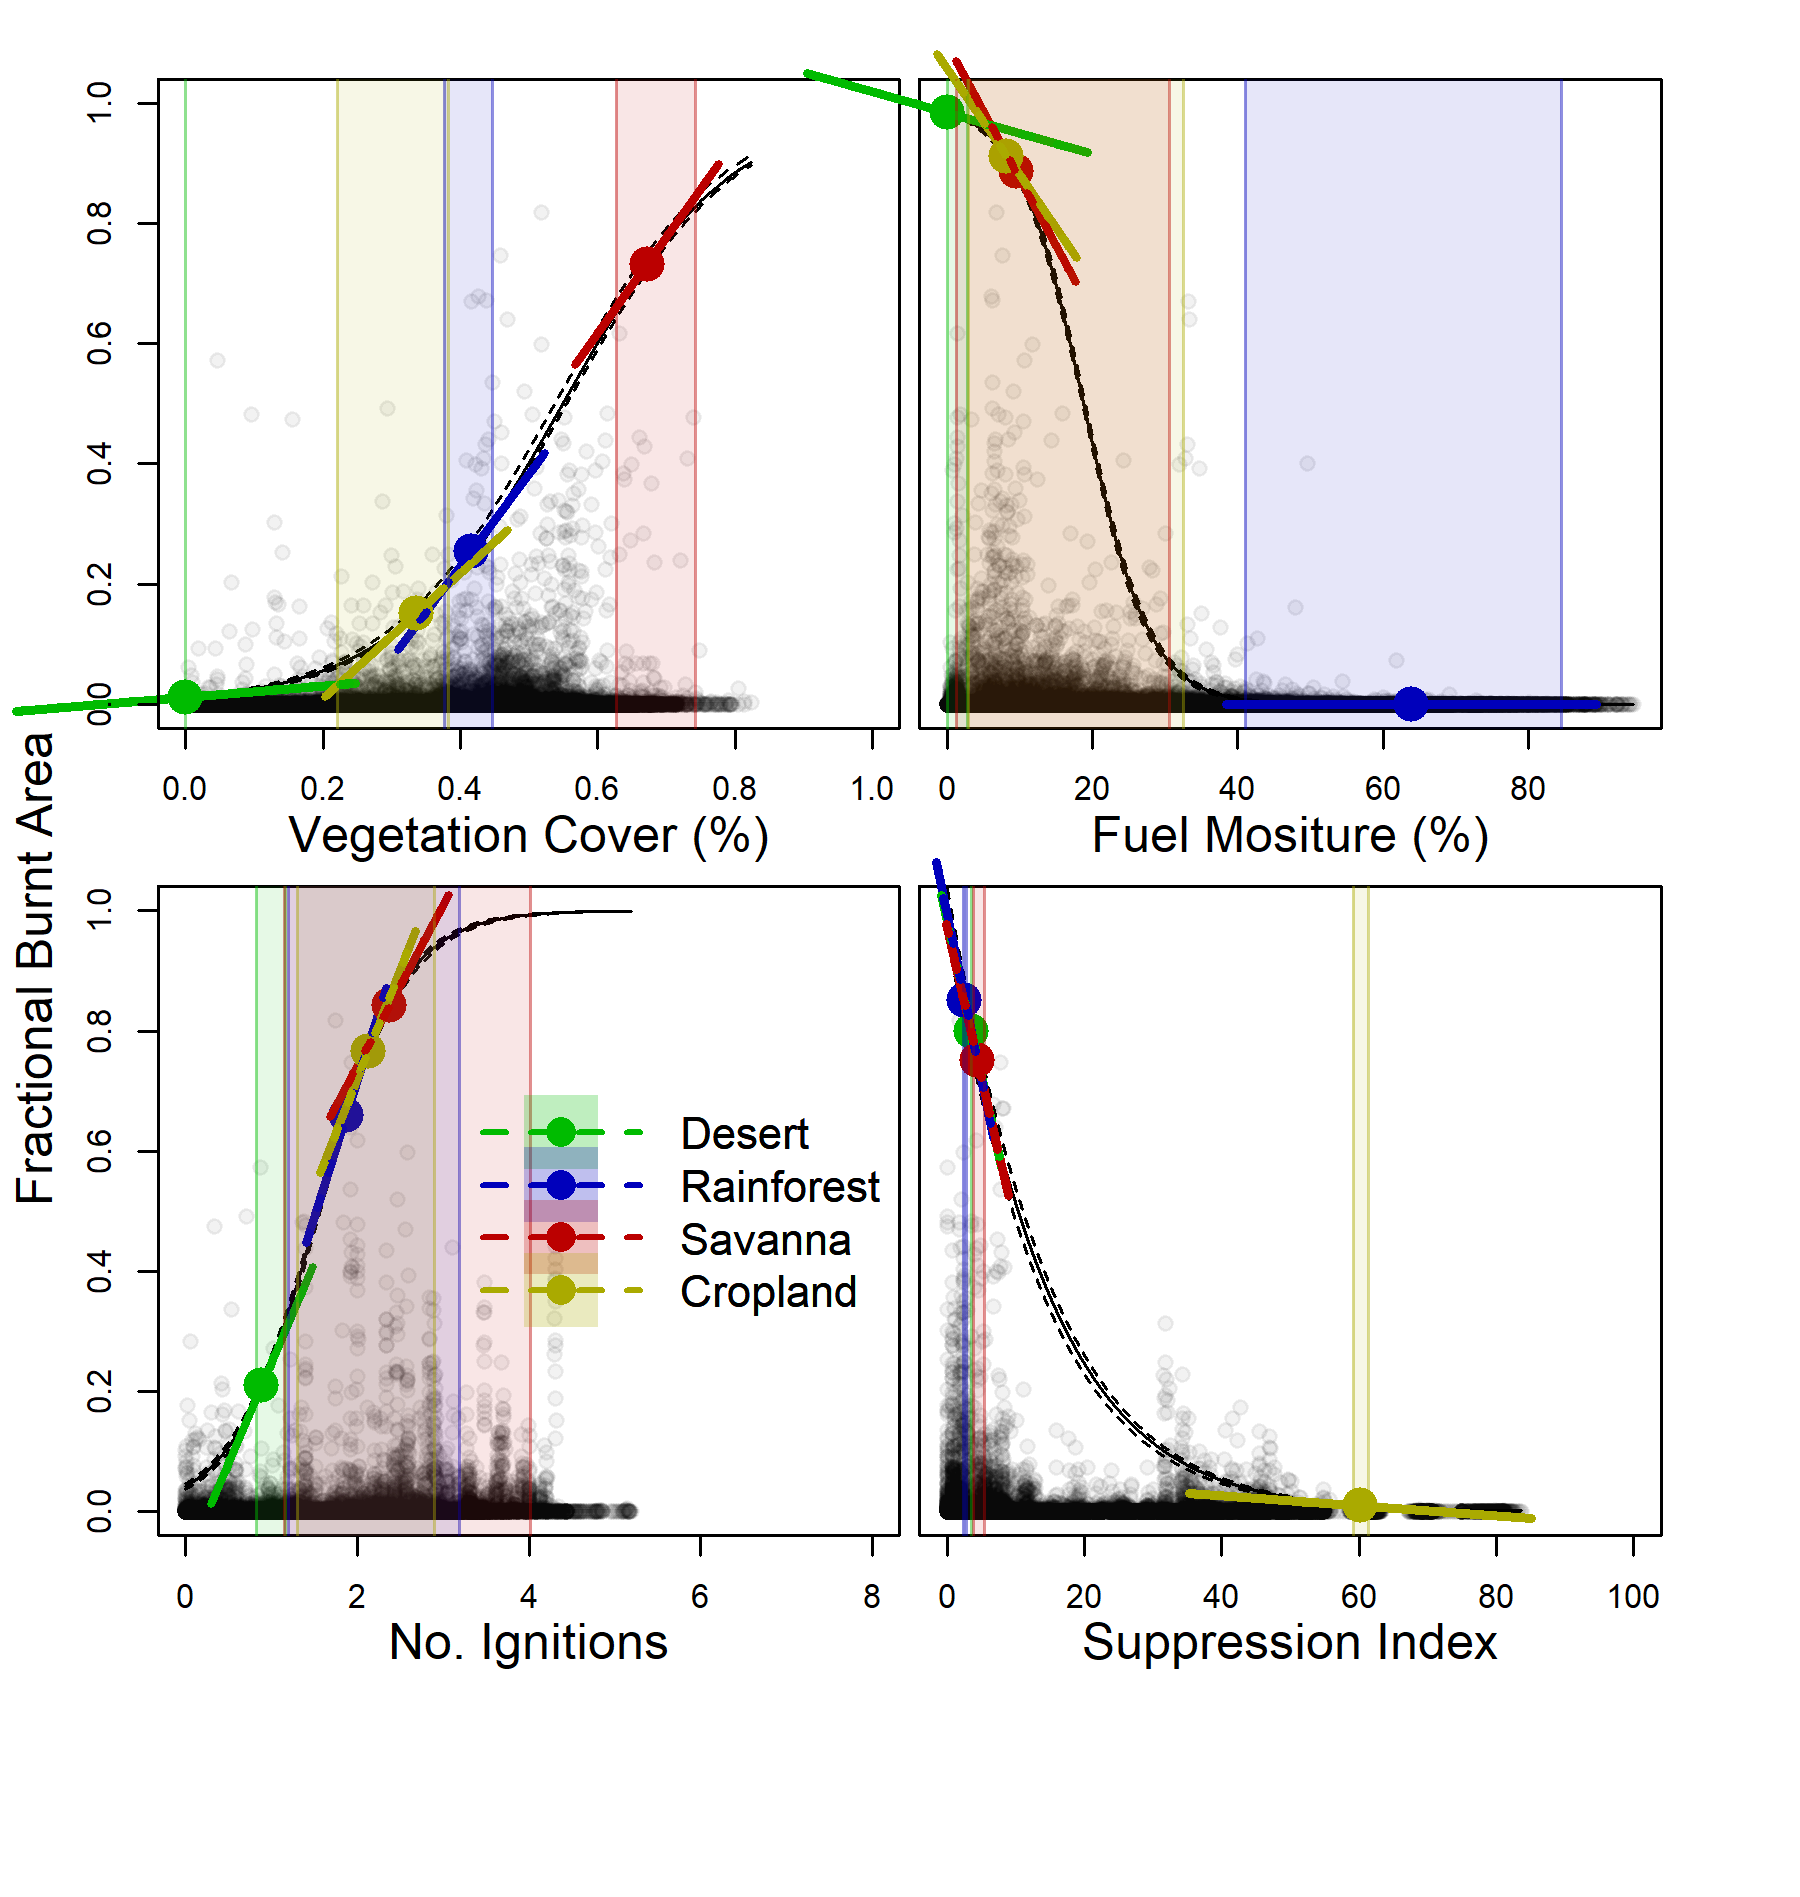
\includegraphics[width=8cm, height=7.0cm,trim={0 1.9cm 0 0}, clip]{images/limitCurves/limLines}
    \end{textblock*}
	\begin{textblock*}{12cm}(7.65cm,2.5cm)
        
\includegraphics[width=13.1cm,trim={0 0 5cm 0}, clip]{images/RawPotSen}	
	\end{textblock*}
\end{frame}


\controlsLines[limLines-Desert-]{Desert/fireMap}
\controlsLines[limLines-Desert-shifted-]{Desert/fireMap}

\begin{frame}
	\frametitle{Controls on fire}
	\begin{textblock*}{12cm}(0.0cm,2.5cm)
        
\includegraphics[width=14cm,trim={0 0 0cm 0}, clip]{images/RawPotSen}	
	\end{textblock*}
\end{frame}

\begin{frame}
	\frametitle{Controls on fire}
	\begin{textblock*}{12cm}(0.0cm,2.5cm)
        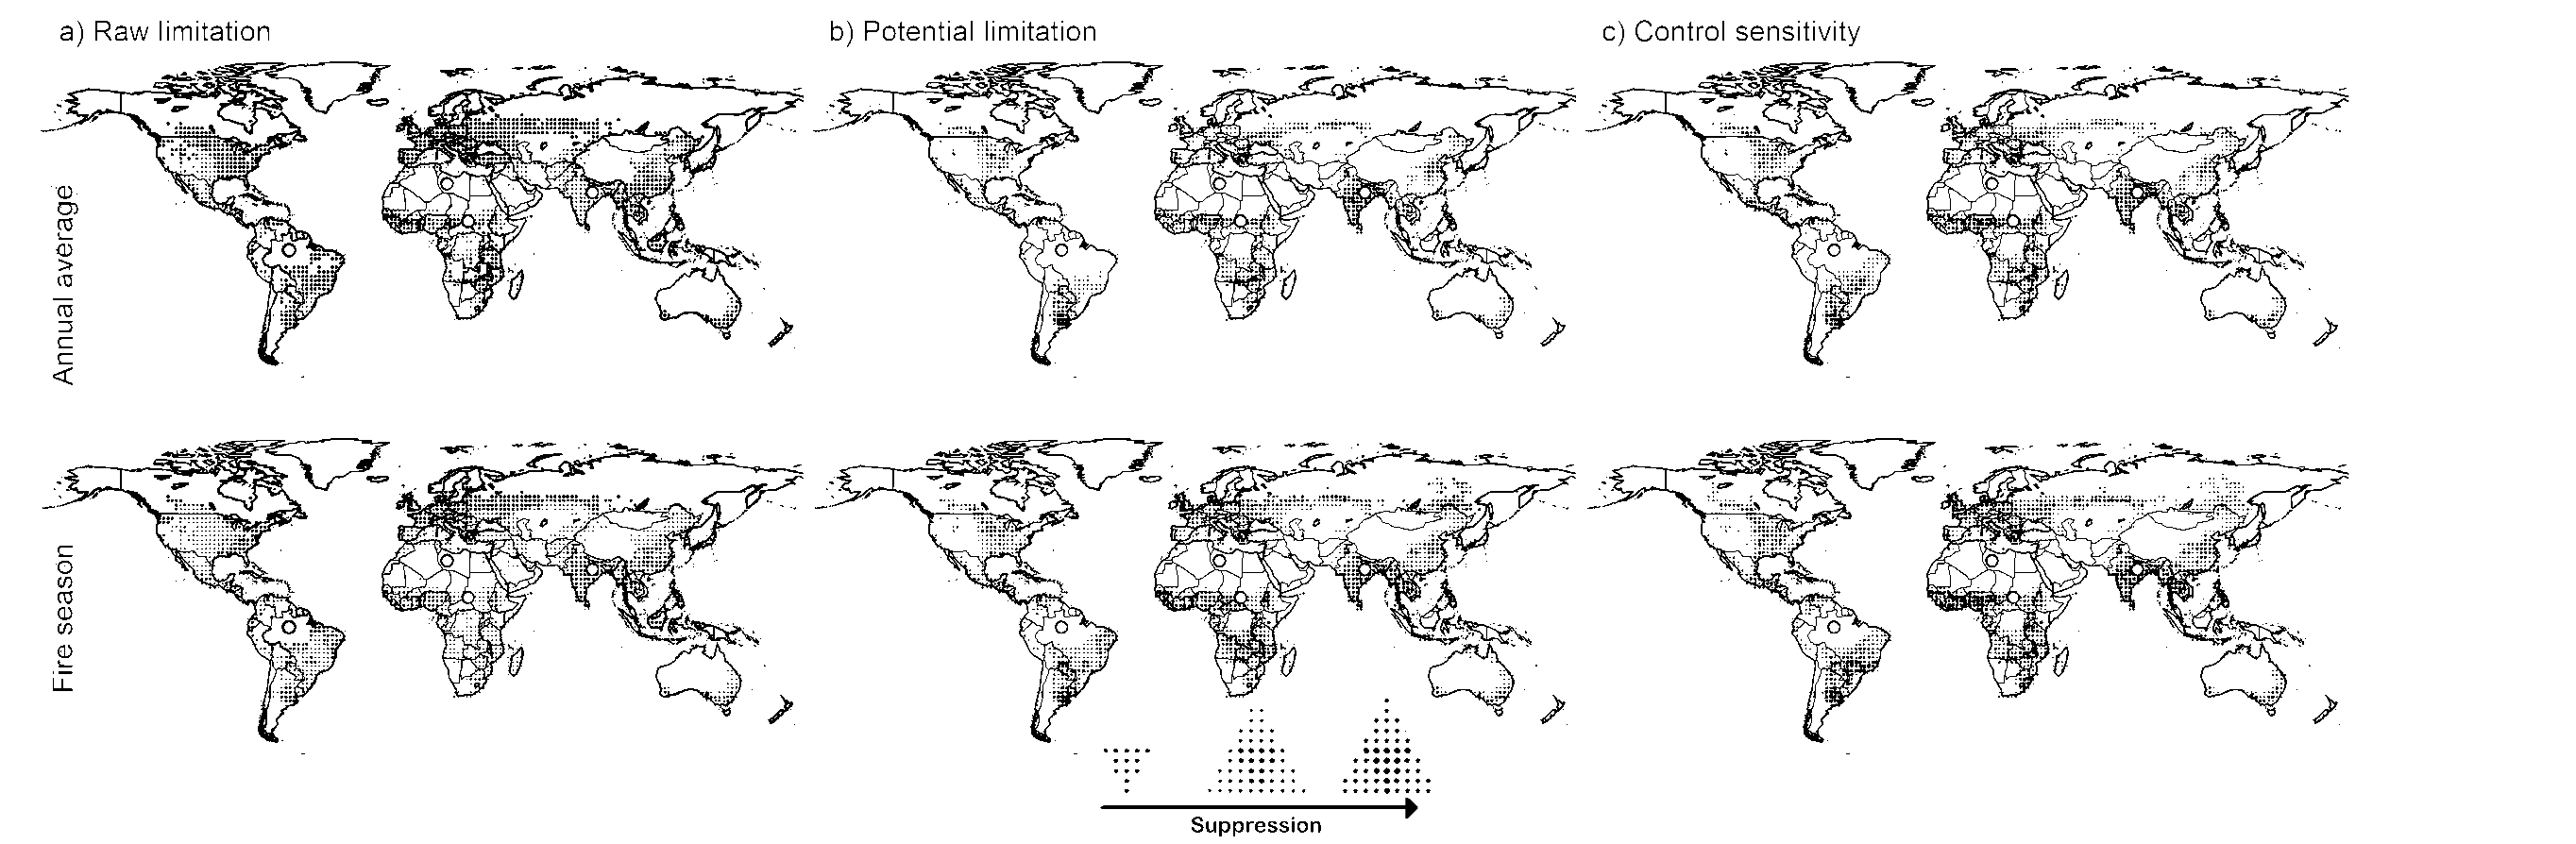
\includegraphics[width=14cm,trim={0 0 0cm 0}, clip]{images/RawPotSen-BW}	
	\end{textblock*}
\end{frame}


